\documentclass[14pt]{beamer}
\usepackage{beamerthemesplit}
\usepackage{apalike}
\usepackage{multirow}
\usepackage{rotating}
\usepackage{booktabs}
\usepackage{hyperref}
\usepackage{graphics}

%\newcommand{\mega}{\fontsize{100}{100}\selectfont}

\usetheme{boxes}
%	\usecolortheme{seahorse}
	\usecolortheme{dove}

\definecolor{McGold}{RGB}{255, 213, 32}
\definecolor{McGreen}{RGB}{ 0, 106, 83}
\setbeamercolor{title}{fg=McGreen, bg=McGold}
\setbeamercolor{frametitle}{fg=McGreen}
\setbeamercolor{structure}{fg=McGreen}

\hypersetup{colorlinks, urlcolor=McGreen}
\hypersetup{colorlinks, linkcolor=McGreen}





\title[$\pi^$]{\resizebox{0.25\linewidth}{!}{\itshape $\pi^*$}}
\author{\href{https://pds.ceu.hu/medzihorsky}{Juraj Medzihorsky}}
\institute{\href{http://www.ceu.hu}{
\includegraphics[scale=0.15]{CEU_logo_long.pdf}}}
\date{\href{http://muni.cz/}{
\includegraphics[scale=0.2]{munilogo.pdf}}\\12. december 2013}

\begin{document}

\begin{frame}
	\frametitle{\href{http://polberg.ceu.hu/}{ }}
	\begin{center}
		\resizebox{0.75\linewidth}{!}{\itshape {$\pi^*$}}
	\end{center}
\end{frame}


\frame{\titlepage}

\section[Outline]{}
\frame{
\frametitle{Outline}
\tableofcontents
}

\section{Model fit}

\begin{frame}
	\begin{center}
		\href{http://sona-web.wz.cz/img/brno/satelit_brno.jpg}{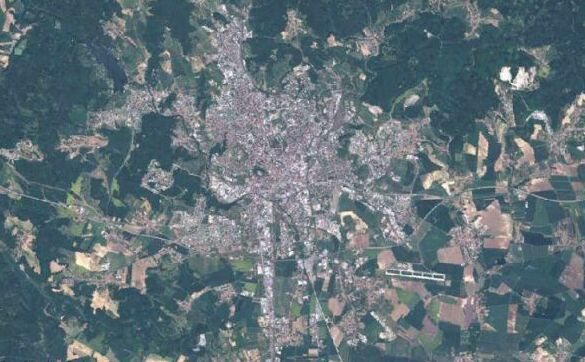
\includegraphics[scale=0.55]{satelit_brno.jpg}}
	\end{center}	
\end{frame}

\begin{frame}
	\begin{center}
		\href{http://clanky.iobchody.com/wp-content/uploads/2007/03/olympia_mapa.jpg}{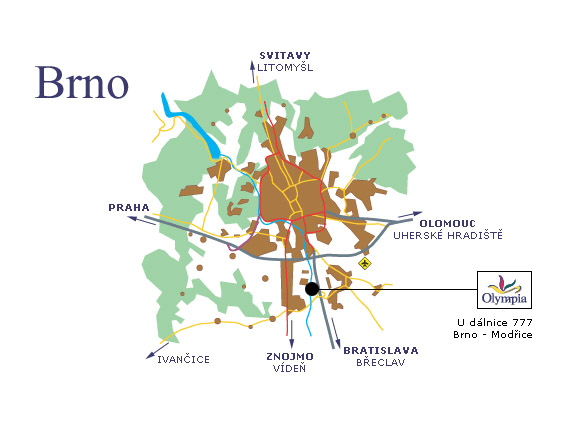
\includegraphics[scale=0.5]{olympia_mapa.jpg}}
	\end{center}	
\end{frame}

\begin{frame}
	\begin{center}
		\href{http://static.bmhd.cz/data/bmhd-archiv/mapy_linek/1974geod.png}{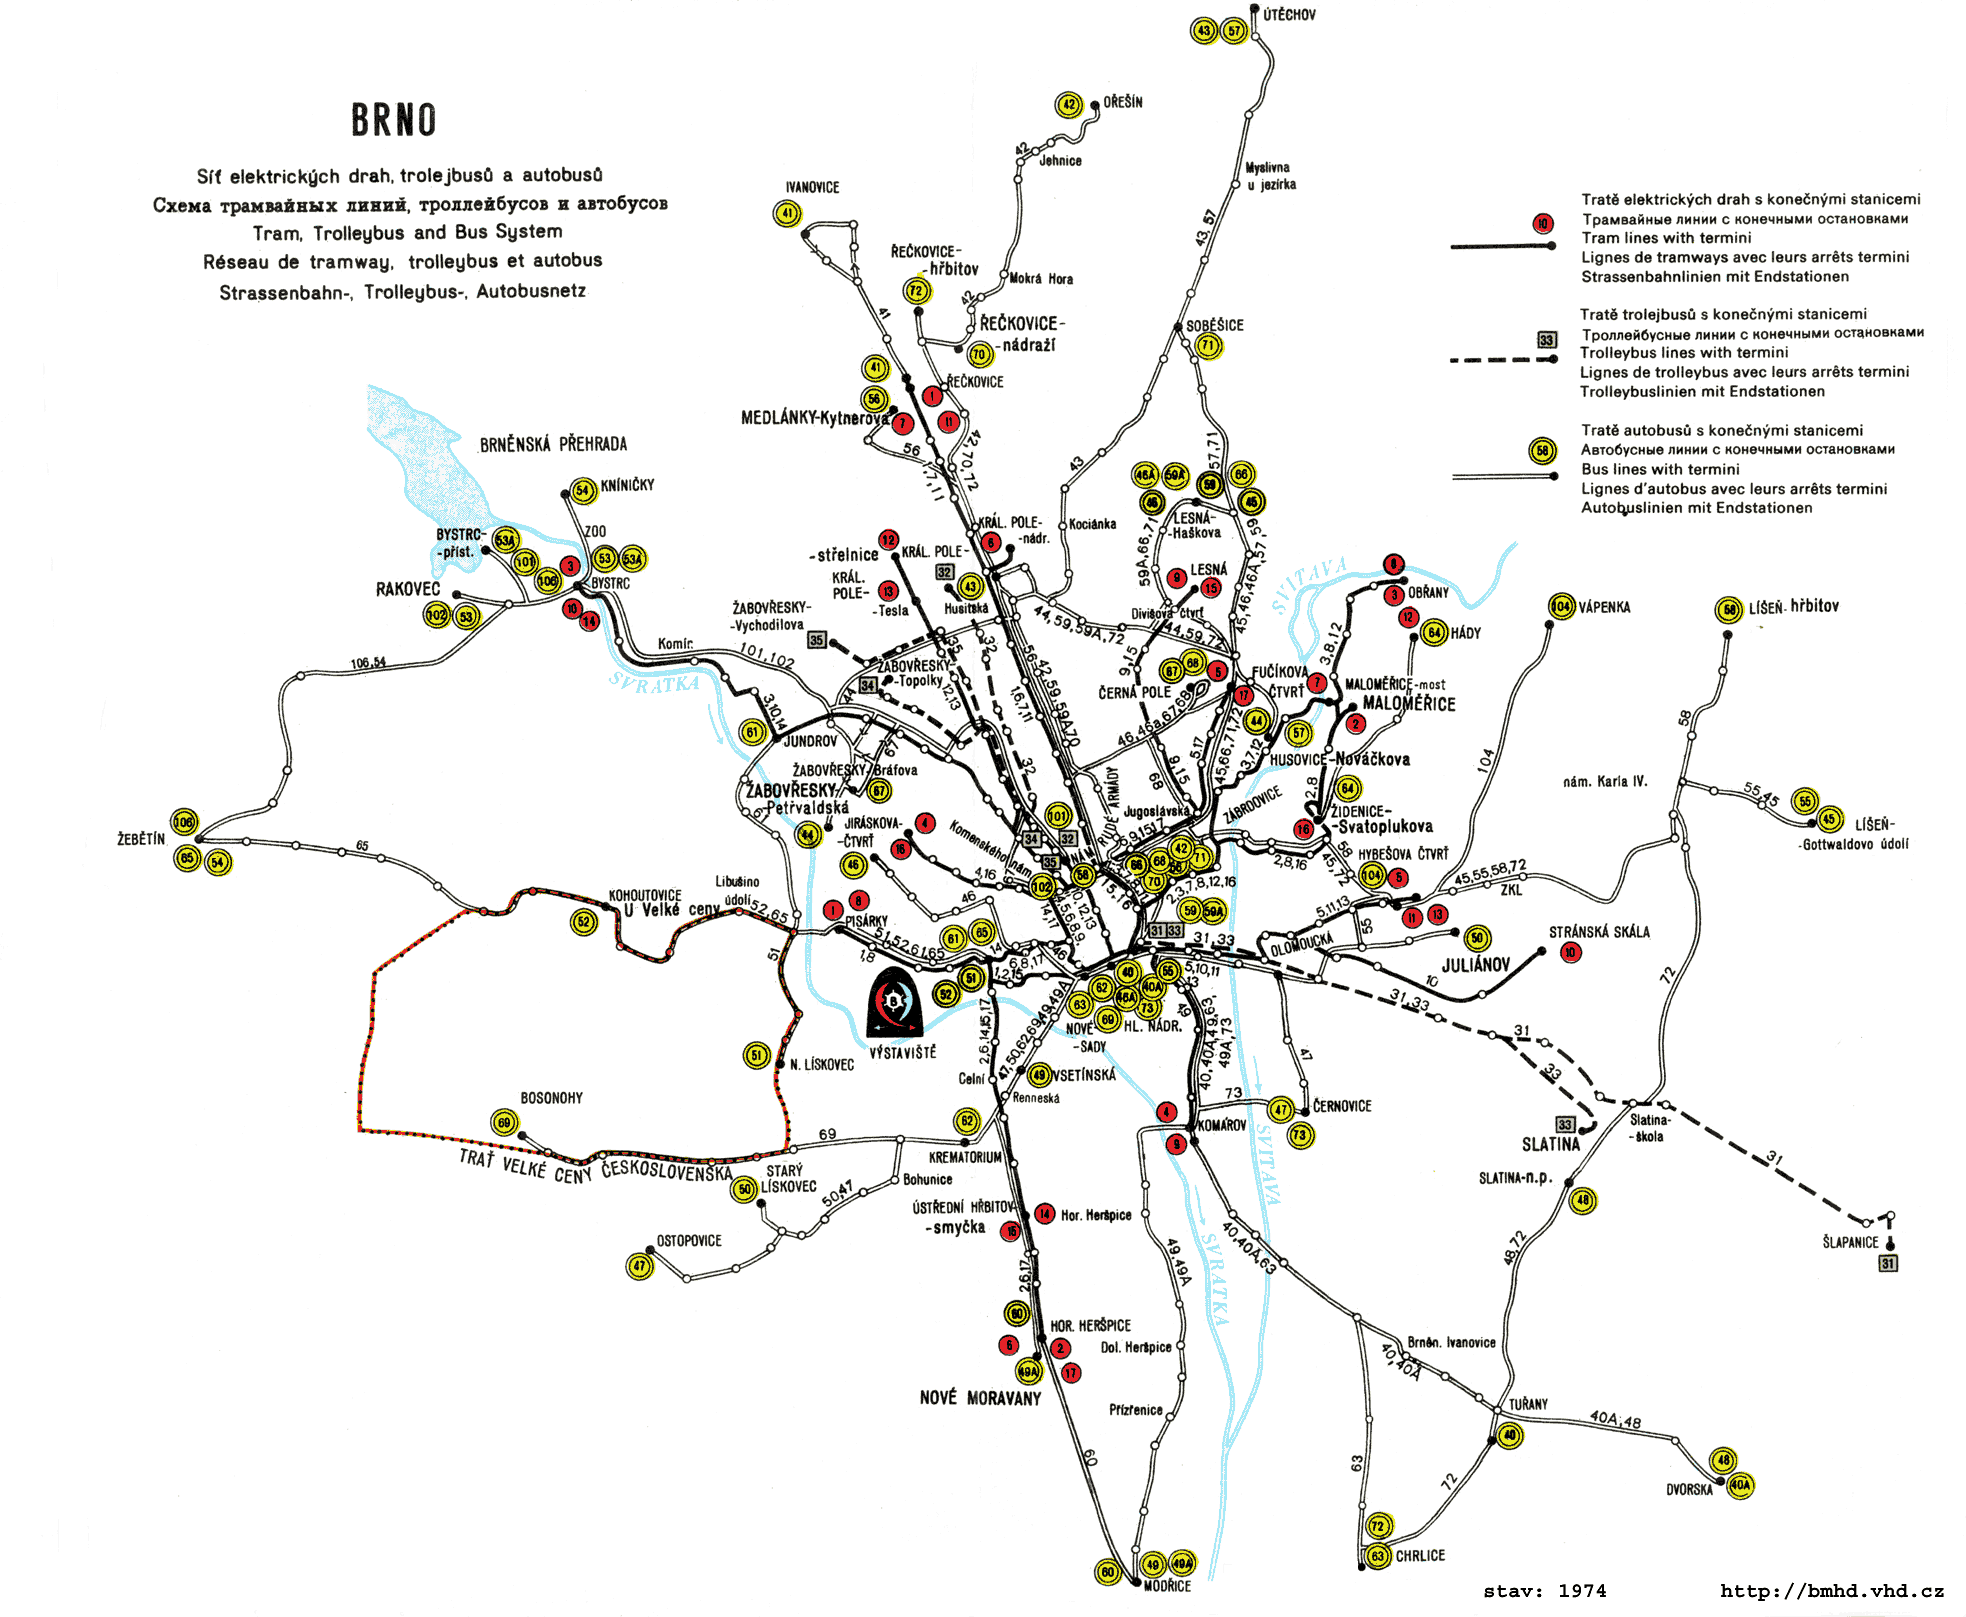
\includegraphics[scale=1.25]{1974geod.png}}
	\end{center}	
\end{frame}

\begin{frame}
	\begin{center}
		\href{http://brno.biskupstvi.cz/petrov/images/mapy/mapa_brno_stred.jpg}{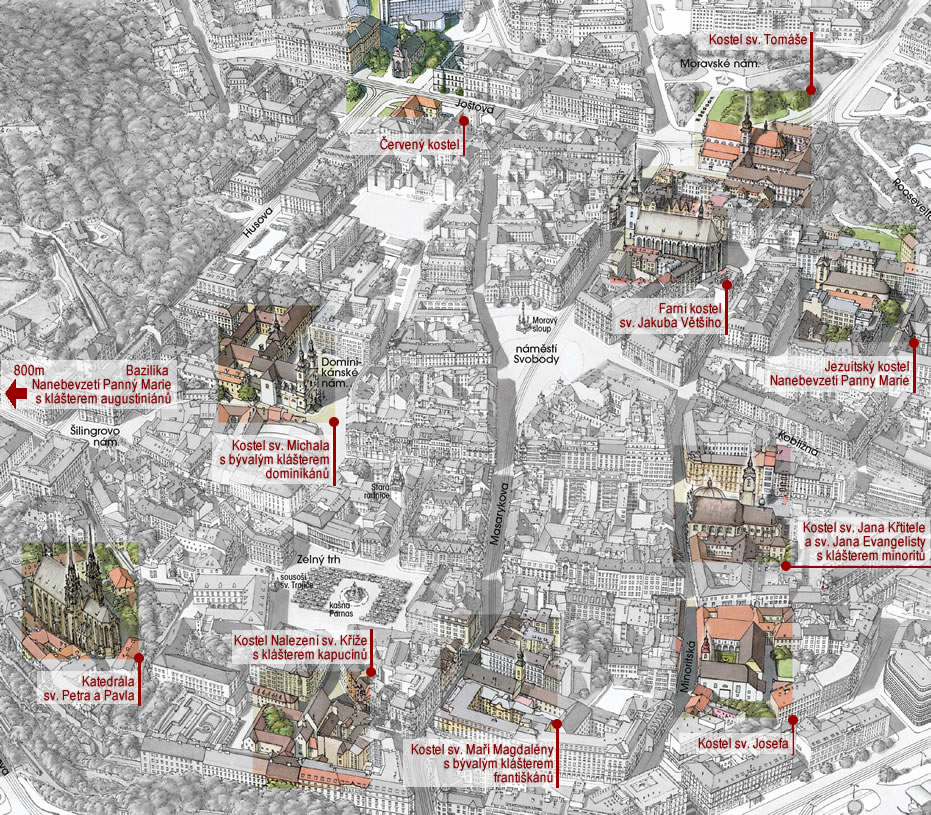
\includegraphics[scale=0.3]{mapa_brno_stred.jpg}}
	\end{center}	
\end{frame}

\begin{frame}
	\begin{center}
		\href{http://www.predseda.org/mapy/mapa-brno.jpg}{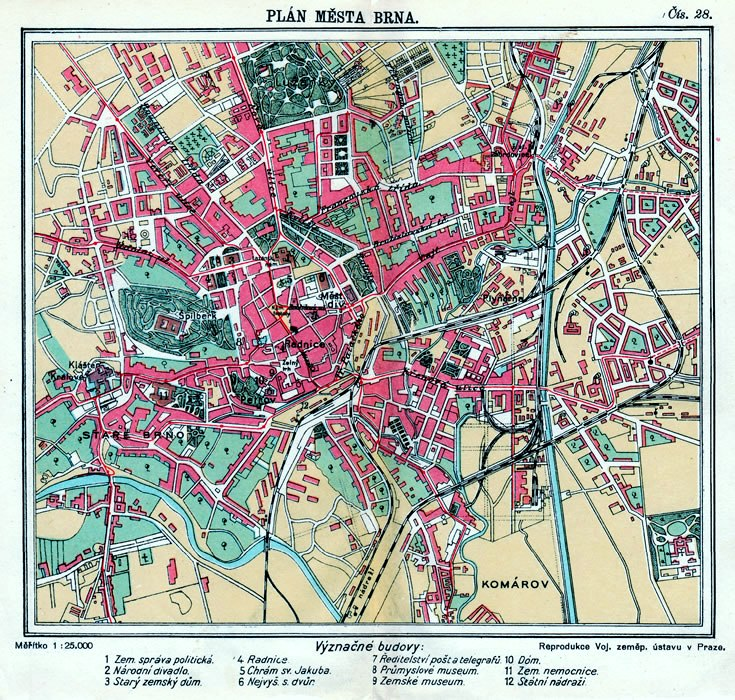
\includegraphics[scale=2]{mapa-brno.jpg}}
	\end{center}	
\end{frame}

\begin{frame}
	\begin{center}
		{\Large Vyhodnocovanie modelov.}
	\end{center}	
\end{frame}




\section{\v{C}o je $\pi^*$}

\begin{frame}
	\frametitle{$\pi^*$}
	\begin{itemize}
		\item[] Rudas-Clogg-Lindsay-ov zmesov\'y index vhodnosti.
		\item[] Miera vhodnosti modelov.
		\item[] Popul\'acia ako zmes dvoch tried:
		\begin{enumerate}
			\item 	trieda pop\'isan\'a modelom;
			\item	trieda nepop\'isan\'a modelom.
		\end{enumerate}
	\end{itemize}
\end{frame}


\begin{frame}
	\frametitle{$\pi^*$}
	\begin{itemize}
		\item[] Hodnota indexu je velkos\v{t} \v{c}asti popul\'acie nepop\'isanej modelom.
		\item[]	Nadob\'uda hodnoty od 0 do 1.
	\end{itemize}
\end{frame}


\begin{frame}
	\frametitle{$\pi^*$}
	\begin{tabular}{rrll}
		$\pi^*({O, \mathcal{M}}) = $ & & & \\
		& $\mathsf{inf}\{\pi\colon$ & $ {O}= (1-\pi){M} + \pi{U},$ & \\
		& & $M \in \mathcal{M},$ & \\
		& & ${U} \ \mathsf{unspecified}$ & $\}$ \\
	\end{tabular}
\end{frame}


\begin{frame}
	\frametitle{$\pi^*$: v\'ypo\v{c}et}
	\begin{itemize}
		\item[] H\v{l}ad\'ame tak\'e hodnoty parametrov modelu, ktor\'e 
				d\'avaj\'u najmen\v{s}iu mo\v{z}n\'u \v{c}as\v{t} popul\'acie
				mimo modelu.	
	\end{itemize}
\end{frame}




\begin{frame}
	\frametitle{$\pi^*$}
	\begin{itemize}
		\item 	Predpoklady v\v{z}dy splnen\'e.
		\item	Priamo\v{c}iary v\'yklad.
		\item 	Nez\'avis\'i od ve\v{l}kosti vzorky.
		\item	Neistotu zh\'r\v{n}a interval spo\v{l}ahlivosti.
		\item 	Nevy\v{z}aduje stochastick\'e vzorky.
		\item 	Umo\v{z}\v{n}uje porovn\'ava\v{t} rozdielne modely.
	\end{itemize}
\end{frame}



\begin{frame}
	\frametitle{$\pi^*$}
	\begin{itemize}
		\item[]	Anal\'yza modelom nepop\'isanej \v{c}as\v{t}i popul\'acie
				ako anal\'yza zbytkov (rezidu\'alov).
	\end{itemize}
\end{frame}





\section{Bal\'ik {\tt pistar}}

\begin{frame}
	\frametitle{{\tt pistar}}
	\begin{itemize}
		\item {\tt R} bal\'ik pre v\'ypo\v{c}et {$\pi^*$}.
		\item Dostupn\'y na \href{https://github.com/jmedzihorsky/pistar}{GitHub-e}.
	\end{itemize}
\end{frame}

\begin{frame}
	\frametitle{\href{http://polberg.ceu.hu/}{ }}
	\begin{center}
		\resizebox{0.75\linewidth}{!}{\itshape {$\pi^*$}}
	\end{center}
\end{frame}





%\begin{frame}
%	\frametitle{Linear regression}
%	\begin{itemize}
%		\item[] $L_{2}^{2}$ linear regression a.k.a OLS
%		\item[] $R^2 = \rho^{2}{(y_o, y_p)}$
%		\item[] $L_{\infty}$ regression a.k.a. minimax or Chebyshev regression
%	\end{itemize}
%\end{frame}



\section{Pou\v{z}itia}


\begin{frame}
	\frametitle{Pou\v{z}itia}
	\begin{itemize}
		\item Jednorozmern\'e modely. 
		\item Viacrozmern\'e norm\'alne rozdelenie.
		\item Modely kontingen\v{c}n\'ych tabuliek. 
		\item Line\'arna a logistick\'a regresia.
	\end{itemize}
\end{frame}



\begin{frame}
	\frametitle{Nov\'y v\'yvoj}
	\begin{itemize}
		\item Zov\v{s}ebecnenie pre ch\'ybaj\'uce d\'ata. 
		\item[] {\small (Rudas 2005, Rudas \& Verdes 2012)}
		\item Bayesovsk\'a verzia.
	\end{itemize}
\end{frame}


\begin{frame}
	\frametitle{\href{http://polberg.ceu.hu/}{ }}
	\begin{center}
		\resizebox{0.75\linewidth}{!}{\itshape {$\pi^*$}}
	\end{center}
\end{frame}


\begin{frame}
	\frametitle{References}
	{\footnotesize
	\begin{itemize}
		\item Rudas, T., Clogg. C., Lindsay, B. (1994) `A New Index of Fit Based on Mixture Methods for the Analysis of Contingency Tables.' {\sl JRSS(b)}. 56(4): 623--639.
		\item Rudas, T. Zwick, R. (1997) `Estimating the Importance of Differential Item Functioning.' {\sl Journal of Educational and Behavioral Statistics}. 22(1): 31--45.

		\item Rudas, T. (1999) `The mixture index of fit and minimax regression.'
{\sl Metrika}. 50: 163--172.
	
		\item Rudas, T. (2005) `Mixture Models of Missing Data.'
{\sl Quality \& Quantity}. 39: 19--36.

		\item Verdes, E., Rudas, T. (2003), `The $\pi^*$ Index as a New Alternative for Assessing Goodness of Fit of Logistic Regression'.
	\end{itemize}
	}
\end{frame}

\begin{frame}
	\frametitle{References}
	{\footnotesize
	\begin{itemize}
		\item Revuelta, J. (2008) `Estimating the $\pi^*$ goodness of fit index for finite mixtures of item response models.' {\sl BJMSP}.  61: 93--113.

		\item Dayton, C.M. (2003) `Applications and computational strategies for the two-point mixture index of fit.' {\sl BJMSP}. 56: 1--13.

		\item Dayton, C.M. (2007) `Applications and extensions of the two-point mixture index of fit.' in: {\sl Advances in Latent Variable Mixture Models}.
	
		\item Knott, M. (2005) `A measure of independence for a multivariate
normal distribution and some connections with factor analysis'. {\sl Journal of Multivariate Analysis}. 96(2): 374--383.

		\item Langeheine, R. (2012) `Konsequenzen des Ignorierens von globalen Modelltests in Studien wie TIMSS, PISA und PIRLS'. in {\sl Item-Response-Modelle
in der sozialwissenschaftlichen Forschung}.

	\end{itemize}
	}
\end{frame}


\end{document}
